\section{Rifrazione aria}
Dopo aver configurato l'apparato sperimentale per l'esperienza di Michelson, abbiamo inserito la cella con la rispettiva pompa.

Anche in questa parte di esperimento è stato necessario contare il numero di frange, effettuato come in precedenza. 

Abbiamo scelto come zero di pressione la pressione atmosferica e ci siamo mantenuti su variazioni alte di pressione al fine di permettere il conteggio delle frange. Riportiamo i $\Delta P$ facendo notare che il riferimento scelto come zero non incide sui dati raccolti, in quanto differenze di valori, mentre riportiamo in seguito i valori medi per le diverse pressioni:
\FloatBarrier
\begin{table}[h!]
\centering
\begin{tabular}{lccccl}
$\Delta P$ (kPa) & \multicolumn{3}{c}{$\Delta N$} &\quad  \overline{\Delta N}\\ \hline 
80            & 17      & 20      & 17      & 18 \\
70            & 16      & 15      & 15      &  15 \\
60            & 13      & 13      & 13      &  13 \\ 
50            & 10      & 10      & 10      &  10 \\
40            & 8       & 8       & 8       & 8 \\ 
\hline\hline
\end{tabular}
\label{tabella 3}
\caption{}
\end{table}
\FloatBarrier
\noindent
Seguendo la relazione \ref{aria} abbiamo eseguito un'interpolazione lineare dei  $\Delta P$ in funzione dei  $\overline{\Delta N}$ ricavando i parametri:
$$
a = 9,045\,\pm 3,352 \qquad    b = 3,981\, \pm 0,252
$$
Tale scelta è stata fatta per permettere di ricavare gli errori su  $a$ e  $b$, utilizzando come errore per le \textit{y} la precisione dello strumento, cioè  $2\,\operatorname{kPa}$. Dai parametri della retta di interpolazione, in particolar modo dal coefficiente angolare, ci è stato quindi possibile ricavare una stima sperimentale dell'indice di rifrazione dell'aria che risulta essere pari a 
$$
\eta_{\text {aria }}= 1,013 \pm 0,252
$$

\begin{figure}[h!]
    \centering
    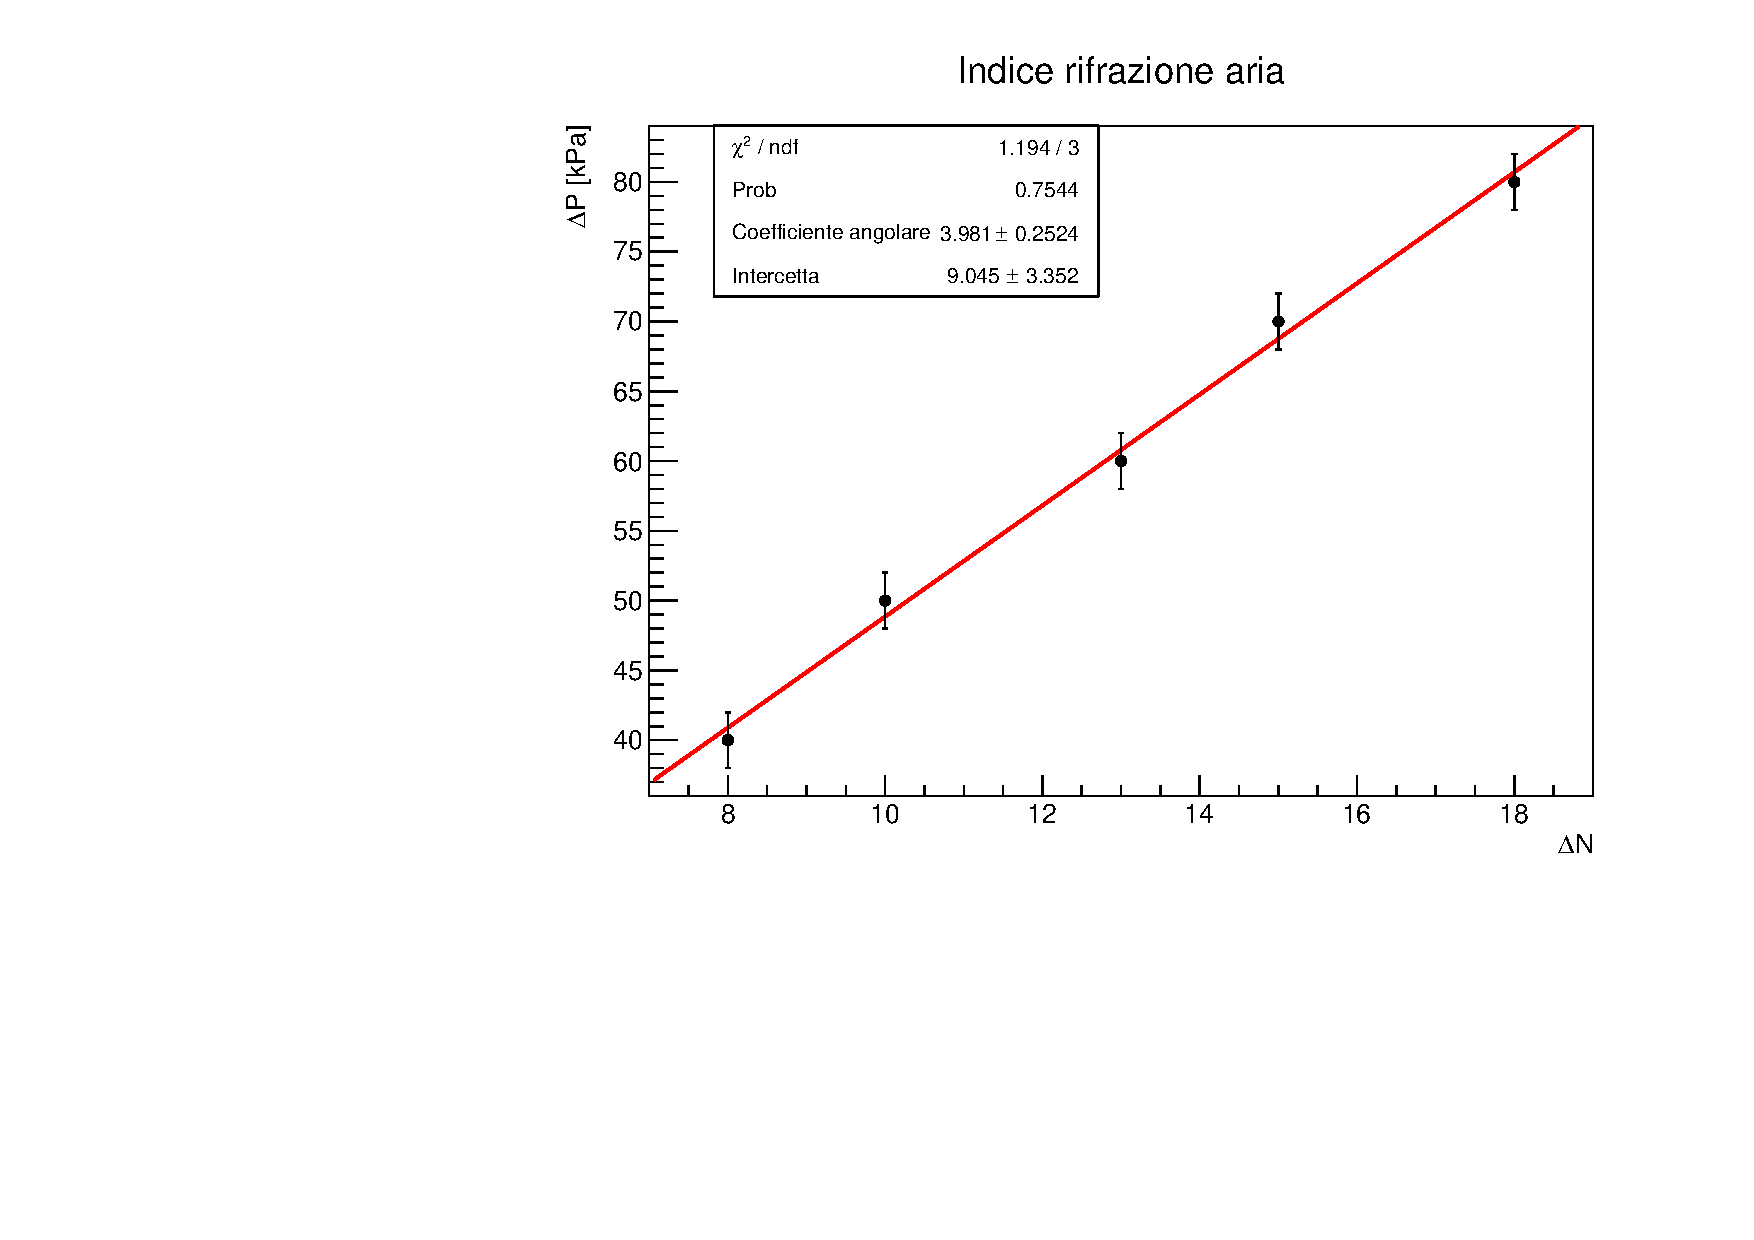
\includegraphics[scale=.6]{immagini/coefficiente aria.pdf}
    \caption{}
    \label{fit aria}
\end{figure}